\documentclass{article}
\usepackage{graphicx}
\usepackage[margin=2.5cm]{geometry}
\usepackage[labelfont=bf]{caption}
\usepackage{color}
\usepackage{xcite}
\usepackage{amsmath}
%\usepackage{natbib}
\usepackage{subcaption}
\usepackage{multirow}

\renewcommand{\textfraction}{1.0}
\renewcommand{\floatpagefraction}{.9}
\newcommand\revised[1]{\textcolor{red}{#1}}
\renewcommand{\topfraction}{0.9}    % max fraction of floats at top
\renewcommand{\bottomfraction}{0.8} % max fraction of floats at bottom
\renewcommand{\textfraction}{0.07}  % allow minimal text w. figs

\makeatletter 
\renewcommand{\thefigure}{S\@arabic\c@figure} 
\renewcommand{\thetable}{S\@arabic\c@table} 

\newcommand{\figdeconv}{2}

\externalcitedocument{betternorm}

\usepackage{url}
\urlstyle{same}

\begin{document}

\begin{titlepage}
\vspace*{3cm}
\begin{center}

{\LARGE
Computing normalization factors for single-cell RNA-seq data: avoiding problems with zero counts
\par}

\vspace{0.75cm}

{\Large 
    \textsc{Supplementary Materials}
\par
}
\vspace{0.75cm}

\large
by

\vspace{0.75cm}
Aaron T. L. Lun$^{1}$, Karsten Bach$^{2}$ and John C. Marioni$^{1,2}$

\vspace{1cm}
\begin{minipage}{0.9\textwidth}
\begin{flushleft} 
$^1$Cancer Research UK Cambridge Institute, University of Cambridge, Li Ka Shing Centre, Robinson Way, Cambridge CB2 0RE, United Kingdom \\[6pt]
$^2$EMBL European Bioinformatics Institute, Wellcome Genome Campus, Hinxton, Cambridge CB10 1SD, United Kingdom \\[6pt]
\end{flushleft}
\end{minipage}

\vspace{1.5cm}
{\large \today{}}

\vspace*{\fill}
\end{center}
\end{titlepage}

\begin{figure}[p]
    \begin{center}
        \begin{minipage}{0.33\textwidth}
            \includegraphics[width=\textwidth,trim=0mm 14mm 2mm 20mm,clip]{../simulations/results/sizeP_1.pdf}
            \includegraphics[width=\textwidth,trim=0mm 14mm 2mm 20mm,clip]{../simulations/results/sizeP_4.pdf}
            \subcaption{}\label{subfig:size_prior}
        \end{minipage}
        \begin{minipage}{0.33\textwidth}
            \includegraphics[width=\textwidth,trim=0mm 14mm 2mm 20mm,clip]{../simulations/results/sizeP2_1.pdf}
            \includegraphics[width=\textwidth,trim=0mm 14mm 2mm 20mm,clip]{../simulations/results/sizeP2_4.pdf}
            \subcaption{}\label{subfig:size_libprior}
        \end{minipage}
    \end{center}
    \caption{
        Performance of DESeq normalization after addition of a pseudo-count.
        A pseudo-count of unity was added to all counts directly (\subref{subfig:size_prior}) or after scaling the pseudo-count by the relative library size (\subref{subfig:size_libprior}), i.e., the pseudo-count added to each cell was equal to the ratio of its library size to the mean library size.
        Simulations were performed with no DE (first row) and varying magnitudes of DE (second row).
        Axes are shown on a log-scale.
        For comparison, each set of size factors was scaled such that the same grand mean across cells was the same as that for the true values.
        The red line represents equality between the rescaled estimates and true factors.
        Cells in the first, second and third subpopulations are shown in black, blue and orange, respectively.
    }
\end{figure}

\section{Resolving linear dependencies in the constructed system}
Consider the application of the deconvolution method on a data set with four cells using a sliding window of size 2.
Assuming cells $j=1$ to $4$ were placed consecutively on the ring, this would yield the linear system
\[
\begin{bmatrix}
1 & 1 & 0 & 0 \\
0 & 1 & 1 & 0 \\
0 & 0 & 1 & 1 \\
1 & 0 & 0 & 1 
\end{bmatrix}
\begin{bmatrix}
\theta_1 \\
\theta_2 \\
\theta_3 \\
\theta_4 
\end{bmatrix}
=
\begin{bmatrix}
\theta_A \\
\theta_B \\
\theta_C \\
\theta_D 
\end{bmatrix}
\]
for pool-based size factor estimates $\theta_A$ to $\theta_D$. 
Assume that the pool-based factors are estimated accurately and precisely, such that the minimum value of the residual sum of squares for this system can be obtained near the set of true values for the cell-based factors.
This system has no unique solution - for the true factors $(\theta_1, \theta_2, \theta_3, \theta_4)^T$, 
    an equally good fit can be obtained with $(\theta_1+x, \theta_2-x, \theta_3+x, \theta_4 - x)^T$ for any real $x$.

The addition of equations relating each $\theta_j$ with its direct estimate $\theta'_j$ ensures identifiability, 
    as a value of $x$ will be chosen that minimizes the residual sum of squares of the $(\theta_1+x, \theta_2-x, \theta_3+x, \theta_4 - x)^T$ from the direct estimates.
In this example, the residual sum of squares for the possible solutions can be written as
\[
\sum_{j \in J_1} (\theta_j +x - \theta'_j)^2+ \sum_{j \in J_2} (\theta_j -x - \theta'_j)^2 
= \sum_{j \in \{J_1, J_2\}} x^2 + 2x\left[ \sum_{j \in J_1} (\theta_j - \theta'_j) - \sum_{j \in J_2} (\theta_j - \theta'_j)\right] + \sum_{j \in \{J_1, J_2\}} (\theta_j - \theta'_j)^2
\]
where $J_1 = \{1, 3\}$ and $J_2=\{2, 4\}$.
For $n=4$ cells in the data set, the above expression is minimized at
\[
x = - \frac{1}{n}\left[ \sum_{j \in J_1} (\theta_j - \theta'_j) - \sum_{j \in J_2} (\theta_j - \theta'_j)\right] \;.
\]
The direct estimate of each size factor is unbiased as stochastic zeroes are not removed, i.e., $E(\theta_j - \theta'_j)=0$.

As the number of cells in the system increases, the sizes of $J_1$ and $J_2$ will increase. 
For example, deconvolution is typically applied in data sets involving at least 200 cells and a sliding window of size 20, such that both $J_1$ and $J_2$ will consist of at least 10 cells.
With more cells, the sum of the errors $\theta_j - \theta'_j$ will approach the sum of their expected values, i.e., zero.
This means that the minimum residual sum of squares will be obtained at $x=0$, i.e., solving the linear system will yield the true values of the size factors.
Thus, the additional equations will not affect accurate estimation of the size factors in the deconvolution method.



\begin{figure}[bt]
    \begin{center}
        \includegraphics[width=0.5\textwidth]{pics/library_ring.pdf}
    \end{center}
    \caption{
        Ring arrangement of cells ordered by library size.
        Each circle represents a cell where the size of the circle corresponds to the library size of that cell.
        Even- and odd-ranking cells lie on opposite sides, with the largest and smallest libraries at the top and bottom, respectively.
        Cells lying in a window of length 4 are highlighted in red.
        Different instances of the window are obtained by sliding the window across the ring.
    }
    \label{fig:library_ring}
\end{figure}

\section{Implementation details of the clustering approach}
Let $\rho_{xy}$ denote Spearman's rank correlation coefficient between the counts of cells $x$ and $y$.
We define the distance between these cells as $1-\rho_{xy}$.
In this manner, a distance matrix is constructed between all pairs of cells.
Hierarchical clustering is performed on this matrix using Ward's clustering criterion.
A dynamic tree cut is used to define clusters of cells using the dynamicTreeCut package v1.62 ({https://cran.r-project.org/web/packages/dynamicTreeCut/index.html}).
This ensures that each cluster contains a minimum number of cells (200 by default) required for stable deconvolution.
Correlation-based clustering is appealing as they are insensitive to global scaling of the expression values in each cell.
Prior normalization is not required, which avoids a circular dependence between normalization and clustering.
Alternatively, one can use known aspects of the data set as clusters, e.g., groupings, batches.
Empirical clustering may not be required if such information is available, which reduces computational work and avoids potential errors.

% While PCA does mean-centering of each gene, this is probably unwise for correlation-based clustering. 
% Two cells that are similar to the mean expression profile will have uncorrelated residuals and would appear to be unrelated. 
% The correct correlation should be near unity as their expression values would match up perfectly. 
% Use of uncentered counts is also easier to interpret and ensures insensitivity to normalization.

By default, the baseline pseudo-cell is chosen from the cluster where the mean library size per cell is equal to the median of the mean library size across all clusters
    (or, for an even number of clusters, the cluster with the smallest mean library size above the median).
This uses the mean library size as a rough proxy for cell similarity.
The baseline cluster is likely to be least dissimilar to every other cluster, which reduces the amount of DE during pairwise normalization between pseudo-cells.
More intelligent choices of the baseline can be used if the similarities between clusters are known, e.g., from visualization after dimensionality reduction.

In general, cluster-specific normalization requires some caution.
Done incorrectly, this may introduce artificial differences between cells in different clusters, 
    such that the statistical rigour of downstream analyses (e.g., to detect DE between clusters) would be compromised.
However, such problems are avoided here by using a two-step normalization strategy.
The first normalization step removes any systematic differences between cells in each cluster, 
    while the second normalization between pseudo-cells removes any differences between clusters.
The end result is that differences between all cells in all clusters are removed.
This is equivalent to the outcome of a hypothetical one-step method that does not use cluster information (and is robust to DE and stochastic zeroes, unlike existing methods).
Moreover, normalization accuracy in Figure~\figdeconv{} is unaffected by the use of clustering prior to deconvolution, which suggests that this approach is valid.

Systematic zeroes within each cluster are also removed prior to deconvolution in that cluster.
This removes genes that have only zero counts across all cells in the cluster.
Such genes provide no information for normalizing between cells in the same cluster, and their removal will not affect the cluster-specific size factor estimates.
However, these genes are retained during rescaling of the size factors between clusters.
This is because they will have non-zero counts in at least one cluster (assuming that systematic zeroes across the entire data set have already been removed).
Removal of such genes will distort the median ratio between pseudo-cells and lead to biased size factor estimates, as described previously for the existing methods.

\section{Deconvolution is inconsistent with spike-in normalization}
The brain data set also contains counts for ERCC spike-in genes that are commonly used for normalizing scRNA-seq data.
Briefly, a constant quantity of spike-in RNA is added to each cell and processed with the cellular RNA \cite{stegle2015computational}.
Upon sequencing and quantification, differences in the coverage of spike-in genes between cells are interpreted as cell-specific biases and removed.
At its simplest, spike-in normalization uses the total count across the spike-in genes as the size factor for each cell.
This is similar to library size normalization with the counts for the cellular genes, but is more robust as no DE is expected across cells for a constant spike-in set.
Problems with stochastic zeroes are avoided, and the assumption of a non-DE majority is not required.
However, spike-in normalization does assume that the same quantity of spike-in RNA can be added to each cell \cite{robinson2010scaling,marinov2014singlecell}.
It also assumes that the spike-ins behave similarly to the cellular transcripts \cite{grun2015design}.
Violations of these assumptions may compromise performance, as observed in some bulk RNA-seq data sets \cite{risso2014normalization}.

Examination of the data indicates that no correlation -- qualitative or quantitative -- 
    exists between the sets of size factors from spike-in and the other normalization methods (Figure~\ref{fig:real_spike}).
This is attributable to the differences in the underlying assumptions of each method.
If most genes are DE, deconvolution and the existing methods will be incorrect and spike-in normalization will be more accurate.
Conversely, spike-in normalization will be incorrect if spike-ins are not added precisely or if spike-in and cellular transcripts behave differently during library preparation.
These results suggest that the validity of each assumption requires some consideration before normalization.
For example, the similarity of the input cell types can be used to gauge the appropriateness of the non-DE assumption. 
Here, over half of the cells are classified as neuronal \cite{zeisel2015brain}, so a non-DE majority of genes is not entirely unreasonable.
Obviously, the truth of each assumption is largely unknown, so it is difficult to definitively determine the correct method for any given data set.

\begin{figure}[btp]
\begin{center}
    \begin{minipage}{0.33\textwidth}
        \includegraphics[width=\textwidth,trim=0mm 5mm 0mm 15mm,clip]{../realdata/Zeisel_ERCCvSF.pdf}
        \subcaption{}\label{subfig:spike_sf}
    \end{minipage}
    \begin{minipage}{0.33\textwidth}
        \includegraphics[width=\textwidth,trim=0mm 5mm 0mm 15mm,clip]{../realdata/Zeisel_ERCCvTMM.pdf}
        \subcaption{}\label{subfig:spike_tmm}
    \end{minipage} \\ 
    \begin{minipage}{0.33\textwidth}
        \includegraphics[width=\textwidth,trim=0mm 5mm 0mm 15mm,clip]{../realdata/Zeisel_ERCCvLib.pdf}
        \subcaption{}\label{subfig:spike_lib}
    \end{minipage} 
    \begin{minipage}{0.33\textwidth}
        \includegraphics[width=\textwidth,trim=0mm 5mm 0mm 15mm,clip]{../realdata/Zeisel_ERCCvDeconv.pdf}
        \subcaption{}\label{subfig:spike_sum}
    \end{minipage}
\end{center}
    \caption{
        Comparisons between the estimated size factors from spike-in normalization to those from (\subref{subfig:spike_sf}) DESeq, (\subref{subfig:spike_tmm}) TMM,
            (\subref{subfig:spike_lib}) library size normalization or (\subref{subfig:spike_sum}) the deconvolution method for all cells in the brain data set.                  
        All sets of size factors were scaled to have a median of unity.
        Axes are shown on a log-scale.
    }
    \label{fig:real_spike}  
\end{figure}

Of greater biological relevance is the fact that spike-in normalization preserves differences in cell size and total RNA content.
In contrast, deconvolution and the existing methods will remove such differences.
This is because they affect all genes within each cell and are subsequently treated as part of the cell-specific bias.
Whether or not this is appropriate depends on whether cell size differences are of interest to the researcher.
In some scenarios, this may be the case such that spike-ins should be used, e.g., when studying cycling cells with differences in total RNA.
For other applications, cell size may be a confounding variable that needs to be removed.
For these data sets, normalization should be performed with the deconvolution method.

Ideally, the decision to use spike-ins or not should be driven by biology, i.e., whether cell size is relevant to the study.
In practice, though, issues such as cost and convenience dictate whether spike-ins are added in the experiment.
This is especially true for the droplet-based protocols \cite{macosko2015highly,klein2015droplet} for which the consistent incorporation of spike-ins is not straightforward.
If spike-ins are not available, normalization of cell-specific biases must be performed with methods that assume a non-DE majority, e.g., TMM, deconvolution.

\begin{table}[p]
    \caption{
        Proportion of the top set of DE genes that were shared between deconvolution and each existing normalization method.
        Top genes were identified as those with the lowest $p$-values from edgeR in the analysis with each normalization method.
        Top sets of size ranging from 100 to 2000 were tested for both the brain and inDrop data sets.
        Smaller sets were not tested due to avoid ambiguous ranks from $p$-values of zero.
    }
    \begin{center}
        \begin{tabular}{l r r r r}
            \hline
            \multirow{2}{*}{\textit{Data set}} & \multirow{2}{*}{\textit{Top}} & \multicolumn{3}{c}{\textit{Method}} \\
                \cline{3-5}
                & & DESeq & TMM & Library size \\
            \hline
            \multirow{3}{*}{Brain}            
            & 100  & 0.44 & 0.60 & 0.71 \\ 
            & 500  & 0.60 & 0.70 & 0.75 \\
            & 2000 & 0.70 & 0.75 & 0.80 \\
            \hline
            \multirow{3}{*}{inDrop}            
            & 100  & 0.88 & 0.94 & 0.98 \\ 
            & 500  & 0.84 & 0.92 & 0.97 \\
            & 2000 & 0.83 & 0.93 & 0.95 \\
            \hline
        \end{tabular}
    \end{center}
\end{table}

\begin{table}[p]
    \caption{ 
        Proportion of the top set of highly variable genes that were shared between deconvolution and each existing normalization method.
        Top genes were identified as those with the largest distance-to-median values. 
        For both data sets, top sets of size between 500 and 2000 were compared between methods.
    }
    \begin{center}
        \begin{tabular}{l r r r r}
            \hline
            \multirow{2}{*}{\textit{Data set}} & \multirow{2}{*}{\textit{Top}} & \multicolumn{3}{c}{\textit{Method}} \\
                \cline{3-5}
                & & DESeq & TMM & Library size \\
            \hline
            \multirow{3}{*}{Brain}            
            & 100  & 0.78 & 0.81 & 0.90 \\ 
            & 500  & 0.78 & 0.80 & 0.88 \\
            & 2000 & 0.67 & 0.73 & 0.84 \\
            \hline
            \multirow{3}{*}{inDrop}            
            & 100  & 0.74 & 0.76 & 0.90 \\ 
            & 500  & 0.57 & 0.59 & 0.85 \\
            & 2000 & 0.59 & 0.61 & 0.85 \\
            \hline
        \end{tabular}
    \end{center}
\end{table}

\end{document}
